\documentclass{article}
\title{The one-ten data}
\usepackage{graphicx}
\usepackage{Statweave}
\begin{document}
\maketitle
The data:
\begin{verbatim}
en 0 2 2  7 6  6   6  6  7  9 9
no 2 0 1  5 4  6   6  6  7  8 9
dk 2 1 0  6 5  6   5  5  6  8 9
nl 7 5 6  0 5  9   9  9 10  8 9
de 6 4 5  5 0  7   7  7  8  9 9
fr 6 6 6  9 7  0   2  1  5 10 9
es 6 6 5  9 7  2   0  1  3 10 9
it 6 6 5  9 7  1   1  0  4 10 8
pl 7 7 6 10 8  5   3  4  0 10 9
hu 9 8 8  8 9  10 10 10 10  0 8
sf 9 9 9  9 9  9   9  8  9  8 0
\end{verbatim}
The SAS code and output:
\begin{Winput}
data lang(type=distance);
	infile "one-ten.dat";
	input lang $ en no dk nl de fr es it pt hu sf;

proc print;

proc cluster method=single outtree=tree;
  id lang;

proc tree horizontal;
  id lang;
\end{Winput}
\begin{Woutput}
Obs    lang    en    no    dk    nl    de    fr    es    it    pt    hu    sf
  1     en      0     2     2     7     6     6     6     6     7     9     9
  2     no      2     0     1     5     4     6     6     6     7     8     9
  3     dk      2     1     0     6     5     6     5     5     6     8     9
  4     nl      7     5     6     0     5     9     9     9    10     8     9
  5     de      6     4     5     5     0     7     7     7     8     9     9
  6     fr      6     6     6     9     7     0     2     1     5    10     9
  7     es      6     6     5     9     7     2     0     1     3    10     9
  8     it      6     6     5     9     7     1     1     0     4    10     8
  9     pl      7     7     6    10     8     5     3     4     0    10     9
 10     hu      9     8     8     8     9    10    10    10    10     0     8
 11     sf      9     9     9     9     9     9     9     8     9     8     0

The CLUSTER Procedure
Single Linkage Cluster Analysis
Mean Distance Between Observations    6.672727

                    Cluster History
                                              Norm    T
                                               Min    i
   NCL    --Clusters Joined---      FREQ      Dist    e
    10    no          dk               2    0.1499    T
     9    fr          it               2    0.1499    T
     8    CL9         es               3    0.1499
     7    en          CL10             3    0.2997
     6    CL8         pl               4    0.4496
     5    CL7         de               4    0.5995
     4    CL5         nl               5    0.7493    T
     3    CL4         CL6              9    0.7493
     2    CL3         hu              10    1.1989    T
     1    CL2         sf              11    1.1989
\end{Woutput}
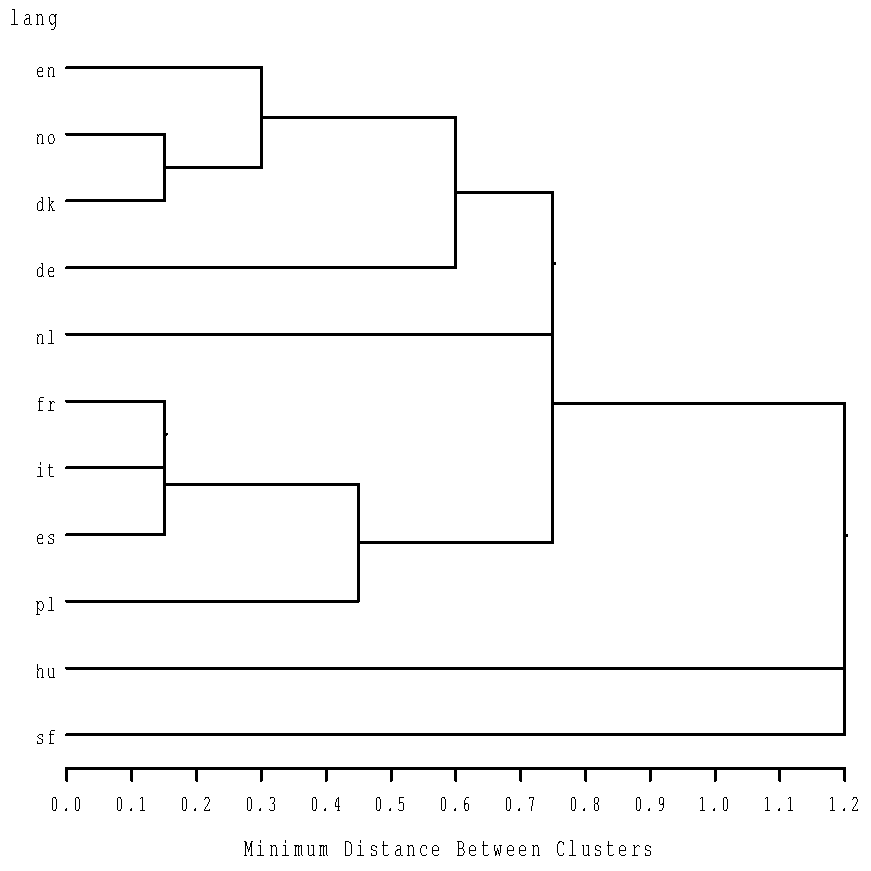
\includegraphics[]{one-ten-1-SAS-fig.pdf}
\begin{Winput}

proc cluster data=lang method=ward outtree=tree2;
  id lang;

proc tree horizontal data=tree2;
  id lang;


run;

\end{Winput}
\begin{Woutput}
The CLUSTER Procedure
Ward's Minimum Variance Cluster Analysis
Root-Mean-Square Distance Between Observations    7.131237

                        Cluster History
                                                              T
                                                              i
   NCL    --Clusters Joined---      FREQ     SPRSQ     RSQ    e
    10    no          dk               2    0.0020    .998    T
     9    fr          it               2    0.0020    .996    T
     8    CL9         es               3    0.0059    .990
     7    en          CL10             3    0.0098    .980
     6    CL8         pl               4    0.0472    .933
     5    nl          de               2    0.0492    .884
     4    CL7         CL5              5    0.1129    .771
     3    hu          sf               2    0.1258    .645
     2    CL4         CL3              7    0.2869    .358
     1    CL2         CL6             11    0.3584    .000
\end{Woutput}
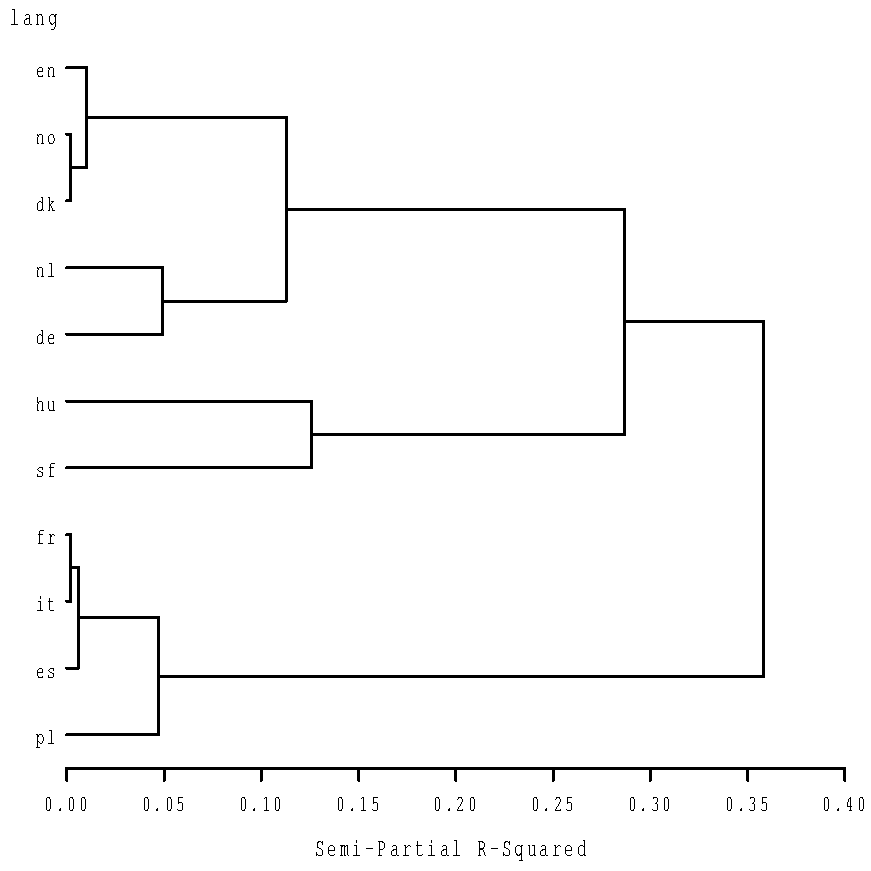
\includegraphics[]{one-ten-2-SAS-fig.pdf}
\end{document}
